\section{Introduction}
\label{sec:introduction}

An enduring problem in machine learning is explaining why a trained 'black box' model behaves as it does. Knowing this is important because it gives insight into the modelling process, and allows users to trust the model outputs as being fair and sensible. As a result, several techniques have been devised to explain the outputs of supervised models. However, these techniques are only usable when there is a target function to be explained, and therefore cannot be used in unsupervised settings. \citet{crabbe2022label} introduced methods for extending existing techniques from the supervised setting to the unsupervised one.  

\vspace{1em}

This paper attempts to replicate and extend the findings of \citet{crabbe2022label}. Specifically, we:
\begin{itemize}
    \item Reproduce the findings of the paper using their provided codebase, and identify which factors (e.g. code quality, clarity of description) hampered or helped this reproduction effort.
    \item Test whether their proposed methods behave consistently on more complex datasets.
    \item Extend their investigation by looking at whether the methods they devised for the unsupervised case are consistent with results obtained when supervision signals are available. 
\end{itemize}

% In \hyperref[sec:scope]{Section 2} we give the necessary mathematical background to understand the authors’ and our own claims and results. In \hyperref[sec:methodology]{Section 3} we describe the specifics of the methodology that we use to test the claims of the authors, both the replication of original experiments and further experiments to test the claims. In \hyperref[sec:results]{Section 4} we show the results of these experiments. In \hyperref[sec:discussion]{Section 5} we discuss what conclusions can be drawn from these experiments about the original claims.

\subsection{Label-Free Explainability for Unsupervised Models}
\citet{crabbe2022label} introduce three broad classes of methods for explaining unsupervised models.

\begin{itemize}
\item \textbf{Feature importance:} feature importance methods aim to describe how each input feature contributes to a given prediction. Mathematically, such a method can be described as a scalar function $a_i(f_j, x)$ which assigns a scalar value to the importance of the $i$th feature of the $j$th output of a model $f$ for a specific input vector $x$.   
There are many existing methods (i.e. possible choices of function $a_i$) for the supervised case (e.g. Lime \cite{ribeiro2016should}, Shap \cite{lundberg2017unified}, Salience \cite{simonyan2013deep}, Integrated Gradients \cite{sundararajan2017axiomatic}), but they cannot be used for unsupervised models because there is no obvious choice of output function $f_j$. \citet{crabbe2022label} argue that any linear feature importance method can be extended to the unsupervised case by substituting the inner product on the latent space for the output function. That is, the score assigned to the $i$th feature for the output of a model $\boldmath{f}$ and sample $\boldmath{x}$ is defined as $b_i(\boldmath{f},\boldmath{x})=a_i(\boldmath{g_x}, \boldmath{x})$ where $\boldmath{g_x(\tilde{x})} \coloneqq \langle \boldmath{f(x)}, \boldmath{f(\Tilde{x}}) \rangle$. 

Intuitively speaking, this method ascribes high importance to features which induce a large change in position in the latent space.

\end{itemize}
Example importance methods describe which elements of the training data were most influential to a particular prediction. These can be further divided into two categories.

\begin{itemize}

\item \textbf{Loss-based example importance:} These methods assess the importance of a given training example to the prediction made for a test example by estimating how the loss function would change if the training example were removed, the model retrained, and new parameters obtained. The authors extend existing methods to measuring the importance of the encoder in an encoder/decoder architecture by only considering loss changes due to the encoder’s parameters.

\newpage{}

\item \textbf{Representation-based example importance:}

For a given test point $\mathbf{x}$, these methods assign an importance score to a training example $\mathbf{x'}$ based on how similar the images $f(\mathbf{x})$ and $f(\mathbf{x'})$ are. The authors argue that these methods do not need any modification to be used in the unsupervised case, since the same procedure can be applied if $f$ maps to a latent space.

\end{itemize}

\section{Scope of reproducibility}
\label{sec:scope}

\citet{crabbe2022label} broadly make three types of claims in their paper. Below we describe each category as well as which hypotheses are specifically tested in each one.

\subsubsection{Area 1: Consistency} They aimed to show that their suggested feature- and example-importance methods identify features and examples that are consistent with a 'sensible' definition of importance. They make two concrete claims in this area.
\begin{itemize}
    \label{claim11}
    \item Claim 1.1: Masking features (i.e. replacing them with a baseline value) identified as the most important by their feature importance method will induce a larger representational shift (change in position in the latent space) than masking features selected at random. 
    \label{claim12}
    \item Claim 1.2: For a given test datapoint, ordering a random set of training datapoints by their unsupervised example importance will place training points of the same class first. 
\end{itemize}

Their other claims relate to the use of their new techniques to study the behaviour of latent representations. 

\subsubsection{Area 2: Correlation}
They train separate latent representations for different tasks, and compare the behaviour of feature- and example- importance methods across the latent representations.

\begin{itemize}
\label{claim21}
\item Claim 2.1: The label-free importance scores assigned to features on the MNIST dataset are moderately correlated across tasks, and there is no evidence that this correlation is lower when comparing supervised and unsupervised models.

\label{claim22}
\item Claim 2.2: Label-free example importance scores have low correlation across different tasks and this correlation is slightly lower when comparing supervised and unsupervised models.
\end{itemize}


\subsubsection{Area 3: Disentanglement} They use their method to study whether disentangled $\beta$-VAE’s (which have a regularisation parameter that penalises correlation between their latent dimensions) see reduced correlations between the importance of a feature to each latent dimension as the regularisation is increased.
\begin{itemize}
\label{claim3}
\item Claim 3: Increasing  $\beta$ does not imply a decrease in correlation between the feature importance scores of separate latent units. 
\end{itemize}
	


\section{Methodology}
\label{sec:methodology}
%Explain your approach - did you use the author's code, or did you aim to re-implement the approach from the description in the paper? Summarize the resources (code, documentation, GPUs) that you used.


To replicate the study, we relied on the public repository provided by the authors. This included scripts to run each of the experiments, which we adapted for our use with minor modifications to fix small errors. We also modified the code for improved parallelisation. The scope and impact of these modifications is described in Appendix \ref{sec:changesincode}. We also conducted some analyses that went beyond their paper. Both the adapted code and our experiments can be found at \url{https://anonymous.4open.science/r/5974660645/README.md}.

\subsection{Model descriptions}
% Include a description of each model or algorithm used. Be sure to list the type of model, the number of parameters, and other relevant info (e.g. if it's pretrained). 

Different models are used depending on the dataset and experiment. The first model is a denoising autoencoder CNN, which is used on MNIST, CIFAR-10 and CIFAR-100. The second model is an LSTM reconstruction autoencoder, which is used on ECG5000. The third model is a SimCLR neural network with a ResNet18 backbone, this model is used for experiments on the CIFAR-10 and CIFAR-100 datasets. The last model is a disentangled $\beta$-VAE, this is used for experiments on MNIST dSprites, CIFAR-10 and CIFAR-100. 

% For MNIST denoising autoencoder CNN, LSTM reconstruction autoencoder on ECG5000, SimCLR neural network with a ResNet18 backbone on CIFAR-10. Disentangeled VAEs are also used on MNIST and dSprites

\subsection{Datasets} 
% For each dataset include 1) relevant statistics such as the number of examples and label distributions, 2) details of train / dev / test splits, 3) an explanation of any preprocessing done, and 4) a link to download the data (if available).

The experiments in the original paper were conducted using four datasets: MNIST, dSprites, ECG5000 and CIFAR-10. For additional experiments CIFAR-100 was used. 

\textbf{MNIST}\cite{lecun1998gradient} consists of 60000 training and 10000 testing images. These images are 28x28 and in greyscale with pixel values ranging from 0 to 255. Each image represents a handwritten digit ranging from 0 to 9, which is also labelled correspondingly. 

\textbf{dSprites}\cite{dsprites17} is a dataset of procedurally generated 2D shapes. These shapes are based on 6 ground truth independent latent factors. The dataset contains 737280 64x64 images with 6 dimensional float64 values of the latent factors. The dataset was split into a training set and a test set, with a ratio of 0.9 for training and 0.1 for the test set.

\textbf{ECG5000}\cite{goldberger2000physiobank} consists of 5000 univariate time series describing the heartbeat of a patient. This is equivalent to around 20 hours of real-time heartbeats. Each time series describes a single heartbeat in 140 time steps. Each heartbeat is also labelled with a 0 or a 1, indicating if the heartbeat is normal(0) or abnormal(1). 4500 time series are used for testing and 400 for training, 100 are used for validation. 

\textbf{CIFAR-10}\cite{krizhevsky2009learning} consists of 60000 32x32 colour images with 10 classes, with 6000 images per class. The dataset is split in 5 training batches and one testing batch, with each batch consisting of 10000 images. Each image contains a label in the form of an integer ranging from 0 to 9.

\textbf{CIFAR-100}\cite{krizhevsky2009learning} is similar to CIFAR-10, the difference is that it contains 100 classes with 600 images for each class. These 100 classes can be grouped together in 20 superclasses. Each superclass is a group of 5 classes, for example: maple, oak, palm, pine, willow form the superclass trees.


\subsection{Hyperparameters}
% Describe how the hyperparameter values were set. If there was a hyperparameter search done, be sure to include the range of hyperparameters searched over, the method used to search (e.g. manual search, random search, Bayesian optimization, etc.), and the best hyperparameters found. Include the number of total experiments (e.g. hyperparameter trials). You can also include all results from that search (not just the best-found results).

The reproduction experiments are conducted using the same model hyperparameters as in the original paper. Table \ref{tab:hyperparams} in the Appendix \ref{sec:apphyper} specifies the hyperparameters for each used model. %For each model the original paper did 20 runs, but due to computational constraints the reproductions are done with 5 runs.




\subsection{Experimental setup and code}
% Include a description of how the experiments were set up that's clear enough a reader could replicate the setup. 
% Include a description of the specific measure used to evaluate the experiments (e.g. accuracy, precision@K, BLEU score, etc.). 
% Provide a link to your code.

\subsubsection{Methodology - Claim 1.1}
This experiment measured the impact of replacing the values of the top-ranked most important features with random baselines. For each of three attribution methods (Saliency, Integrated Gradients, and Gradient SHAP), we calculated unsupervised feature importance values for all features. Then, for various values of $M \in \mathbb{N}$, we replaced (or 'masked') the top $M$ features with a fixed baseline value, and measured the change in position in the latent space. This distance is referred to as the \textit{representation shift}, and is calculated as $||\boldmath{f}_e(\boldmath{x})-\boldmath{f}_e(\mathbf{m}(x))||$ where $f_e$ is our encoder, and $\mathbf{m}$ is our masking function.

\vspace{1em}

The authors hypothesised that if an unsupervised feature attribution method was 'sensible', then masking the top $M$ highest ranked features should always induce a larger representation shift than when the masked features were chosen at random. 

\subsubsection{Methodology - Claim 1.2}
This experiment measured whether, for a given test example $x^*$, the top-ranked most similar training examples were more likely to share class labels with $x^*$. For a given value of $M \in \mathbb{N}$, we computed what proportion of the top $M$ most similar training examples shared the same class label as $x^*$ - this proportion is referred to as the \textit{similarity rate}. We repeated this process for 1000 separate test examples, and averaged the resulting proportions. The authors hypothesised that a 'sensible' example similarity method should see higher values of this proportion at lower values of $M$. 

This process was repeated for each of three datasets (CIFAR-10, MNIST, ECG5000) and five example importance methods (DKNN \citep{crabbe2022label}, SimplEx \citep{Crabbe2021Simplex}, TracIn \citep{pruthi2020estimating}, Influence Functions \citep{koh2020understanding}, CosineNN). The 'CosineNN' method was created by us as a drop-in replacement for DKNN. It uses cosine similarity, rather than inverse distance, to define similarity between train and test points.


\subsubsection{Methodology - Claim 2.1}
This experiment compared feature importance for latent representations trained for different tasks on the MNIST dataset. A model was trained on each of the three unsupervised tasks of reconstruction, denoising, and inpainting, and the supervised task of classification. Label-free gradient Shap was used to score the importance of each feature to each latent representation. Then, we calculated the  Pearson correlation coefficient of the importance scores of matching features between pairs of latent representations. That is, if $\mathbf{f}$ and $\mathbf{g}$ were two encoders corresponding to different latent representations, and $b_i$ the label free gradient Shap of the $i$th feature, we calculated the correlation between   $b_i(\boldmath{f},\boldmath{x})$ and $b_i(\boldmath{g},\boldmath{x})$ across all choices of $i$. 


\subsubsection{Methodology - Claim 2.2}
This experiment had the same structure as 2.1, but measured correlations in example importance (measured using the label-free DKNN method) instead. That is, if $c^n(f, x_m)$ refers to the example importance of the $n$th training point to the $m$th test point, and $\mathbf{f}$, $\mathbf{g}$ referred to encoders learned for different tasks, then we measured the correlation of  $c^n(\mathbf{f}, x_m)$ and $c^n(\mathbf{g}, x_m)$ pooled across all $n$ and $m$.

\subsubsection{Methodology - Claim 3} 
This experiment aimed to use label-free feature importance methods to study the behaviour of disentangled VAEs, a VAE architecture where a regularisation parameter ($\beta$) penalises correlation between variables in the learned latent space. The authors initially hypothesised that this implied that as the parameter was increased, the correlation of label-free feature importance scores between different units should decrease. Ultimately, they found no evidence to support their initial hypothesis. To test this hypothesis, we compute feature importance scores separately for each latent unit, then computed the Pearson correlation coefficient of corresponding scores between the latent units.  

We also attempted to corroborate the authors' explanation for their findings by visualising the behaviour of each latent unit for multiple values of $\beta$ using Lucid \cite{olah2017feature}, a method which determines the input that would maximise the response from each latent unit. 

\subsubsection{Additional Experiment - Extending consistency and task comparison to CIFAR-10 and CIFAR-100}

We repeated the experiments described above on two extra datasets: CIFAR-10 (for which 1.1 and 1.2 were already tested in the original paper) and CIFAR-100 datasets (which is entirely new). We had two aims: first, we wanted to check whether the label-free methods would still be consistent on these more complex datasets. Second, we wanted to check whether there would be a larger difference between the latent representations of models that were trained with and without access to labels, since the labels may provide a more important signal for training representations when the data is more complex. Due to the increased complexity of the task, we also added one extra layer both to the encoder and decoder and increased the network's width. The details of the encoder and decoder networks are described in Appendix \ref{sec:autoencoderarch}. 


\subsubsection{Additional Experiment - Comparison of Unsupervised and Supervised Feature Importance}

We ran an additional experiment to corroborate their claims of \textbf{consistency} for feature importance. Their experiments showed that features with higher importance induced a higher representational shift when masked. However, it's unclear how this representational shift can be interpreted: there's no guarantee that a large shift in the latent space would correspond to a large shift in a target function if one was learned on the latent space.


To answer this question, we examined whether the feature importance scores calculated for a classifier were similar to those calculated for the layers responsible for the latent representation. That is, if the full classifier can be described as the composition of a latent space encoder $f_e$ and a projection head $f_d$, we computed for each test point $x_j$ the correlation $\rho_j$ of $\mathbf{b_i(f_e, x_j)}$ and $\mathbf{b_i(f_d \circ f_e, x_j)}$ across all features $i$. Finally, we averaged $\rho_j$ to obtain a point estimate of the correlation between importance scores of $f_e$ and $f_d \circ f_e$.

We took the classifier that was trained on the MNIST data, and followed the above procedure for three types of feature importance metrics (Gradient Shap \cite{lundberg2017unified}, Salience \cite{simonyan2013deep} and Integrated Gradients \cite{sundararajan2017axiomatic}). We repeated this process across 5 random reseedings of the model. If the unsupervised and supervised feature importance are consistent with each other, we would expect a high correlation.


\subsection{Computational requirements}

In our experiments, we used a single NVIDIA A100 GPU and 8 cores of an AMD EPYC 7643 processor. All together, the experiments took approximately 80 hours to run. 

% Include a description of the hardware used, such as the GPU or CPU the experiments were run on. 
% For each model, include a measure of the average runtime (e.g. average time to predict labels for a given validation set with a particular batch size).
% For each experiment, include the total computational requirements (e.g. the total GPU hours spent).
% (Note: you'll likely have to record this as you run your experiments, so it's better to think about it ahead of time). Generally, consider the perspective of a reader who wants to use the approach described in the paper --- list what they would find useful.

\section{Results}
\label{sec:results}

%Start with a high-level overview of your results. Do your results support the main claims of the original paper? Keep this section as factual and precise as possible, reserve your judgement and discussion points for the next "Discussion" section. 
% We have mostly been able to reproduce the reported experimental results from the original paper. We were able to execute the experiments with the available code with only minor modifications.

% \subsection{Results reproducing original paper}
%For each experiment, say 1) which claim in Section~\ref{sec:claims} it supports, and 2) if it successfully reproduced the associated experiment in the original paper. 
%For example, an experiment training and evaluating a model on a dataset may support a claim that that model outperforms some baseline.
%Logically group related results into sections. 

\subsubsection{Claim 1.1 - Consistency of feature importance}

Our results were closely aligned with those of the original work (Figure \ref{fig:cons_features}). We found that for all models, including those trained on the CIFAR-100 dataset, the representation shift induced by masking high-importance features was always greater than in the random baseline, although in the case of CIFAR-10 this was only true for the Integrated Gradients method. In general, integrated gradients and gradient Shap performed best, while saliency performed worst.


\begin{figure*}[h]
	\vspace{-0.1in}
	\centering
	\subfigure[MNIST]{
		\begin{minipage}[t]{.25\linewidth}
			\centering
			%\includegraphics[width=1\linewidth]{img/og/mnist_consistency_features}
            \includegraphics[width=1\linewidth]{img/rp/mnist_consistency_features}    
		\end{minipage}%
	}%
	\subfigure[ECG5000]{
		\begin{minipage}[t]{.25\linewidth}
			\centering
			%\includegraphics[width=1\linewidth]{img/og/ecg5000_consistency_features}
            \includegraphics[width=1\linewidth]{img/rp/ecg5000_consistency_features}
		\end{minipage}%
	}%
	\subfigure[CIFAR-10]{
		\begin{minipage}[t]{.25\linewidth}
			\centering
			%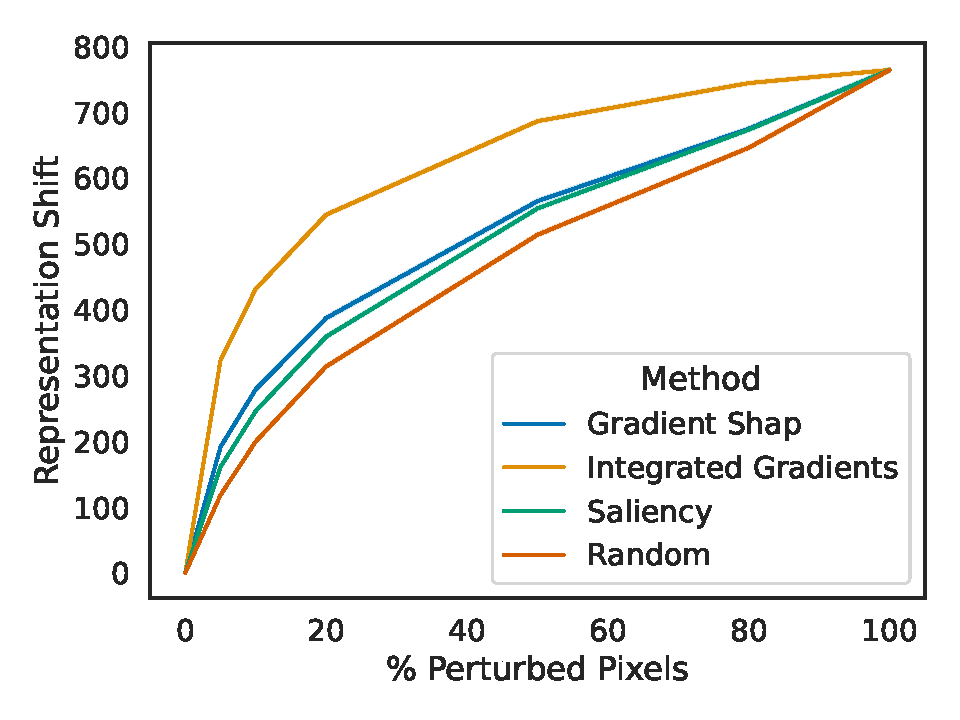
\includegraphics[width=1\linewidth]{img/og/cifar10_consistency_features}
            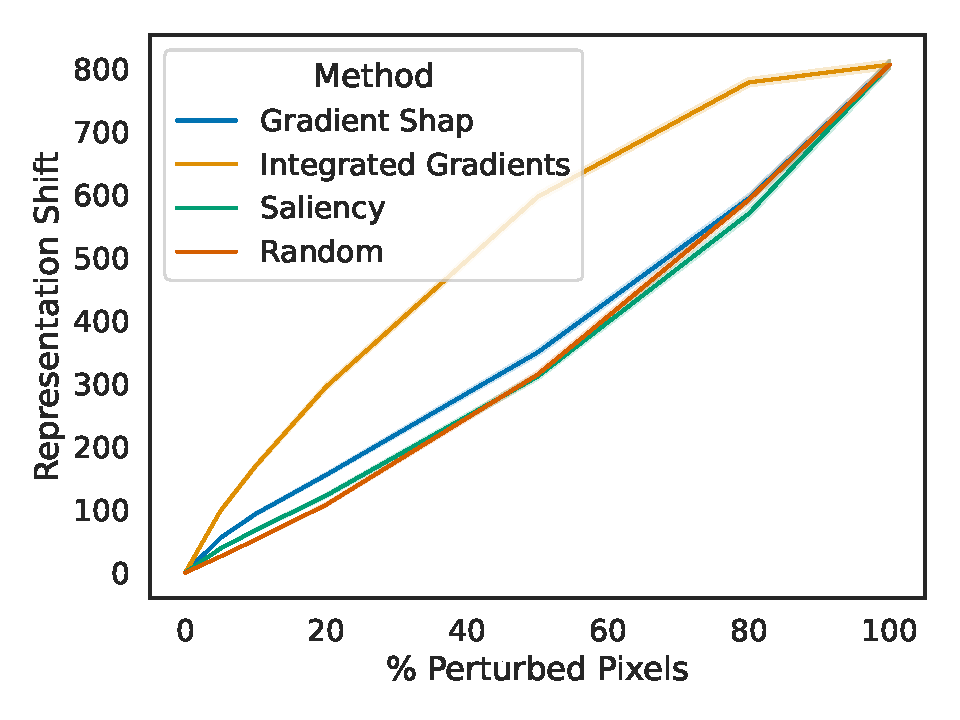
\includegraphics[width=1\linewidth]{img/rp/cifar10_consistency_features}
		\end{minipage}%
	}%
    \subfigure[CIFAR-100]{
		\begin{minipage}[t]{.25\linewidth}
			\centering
			%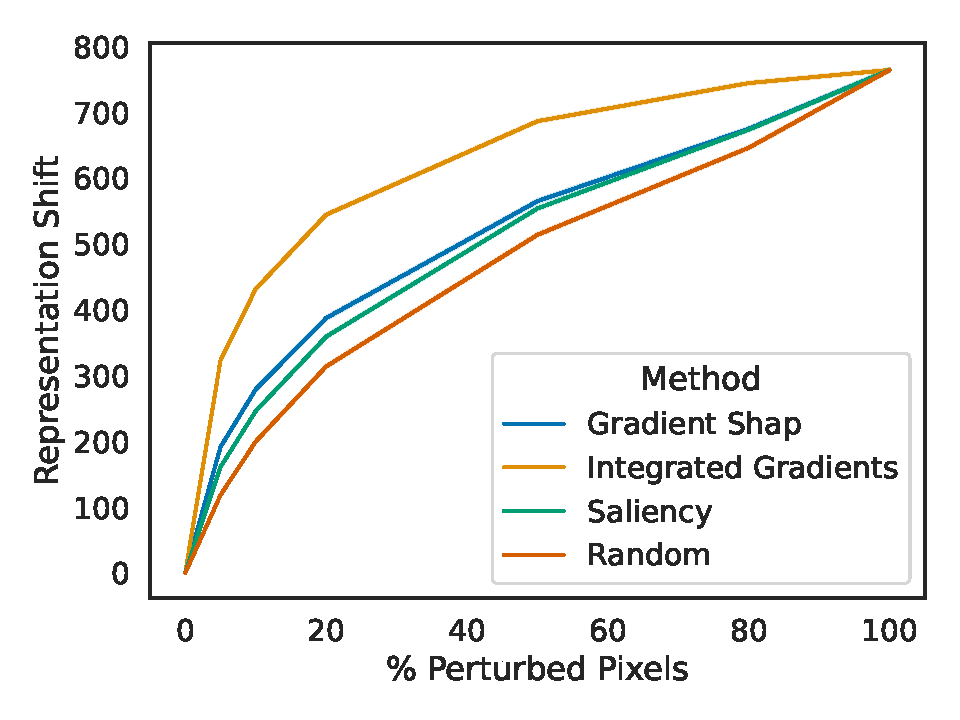
\includegraphics[width=1\linewidth]{img/og/cifar10_consistency_features}
            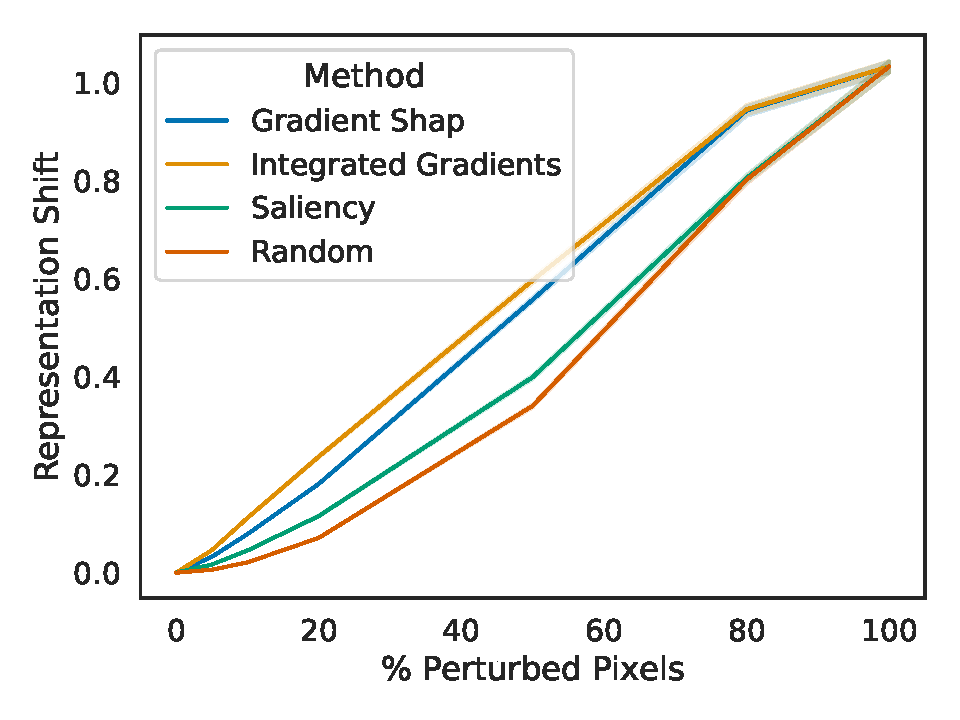
\includegraphics[width=1\linewidth]{img/extra/cifar100_consistency_features}
		\end{minipage}%
	}%
	\vspace{-0.1in}
	\caption{Consistency check for label-free feature importance. Each curve shows the size of representation shift that is induced as we mask an increasing percentage of the top-ranked most important features. Each line shows the average and $95 \%$ standard deviation over 5 random reseedings.}
	\label{fig:cons_features}
	\vskip -0.2in
\end{figure*}

\subsubsection{Claim 1.2 - Consistency of example importance}


Our experiments replicated the findings of \citet{crabbe2022label} (Figure \ref{fig:cons_examples}{}). Similarity rates were always higher when calculated across examples with higher label-free example importance, including on the CIFAR-100 dataset. The one exception to this was the SimplEx method on ECG5000, where high-importance examples only achieved marginally higher similarity than the lowest importance scores. This is directionally in line with the results of \citet{crabbe2022label}, but it was not remarked on in their paper. Our newly defined 'cosine nearest neighbours' techniques outperformed all other methods.


\begin{figure*}[]
	\vspace{-0.05in}
	\centering
	\subfigure[MNIST]{
		\begin{minipage}[t]{.25\linewidth}
			\centering
			%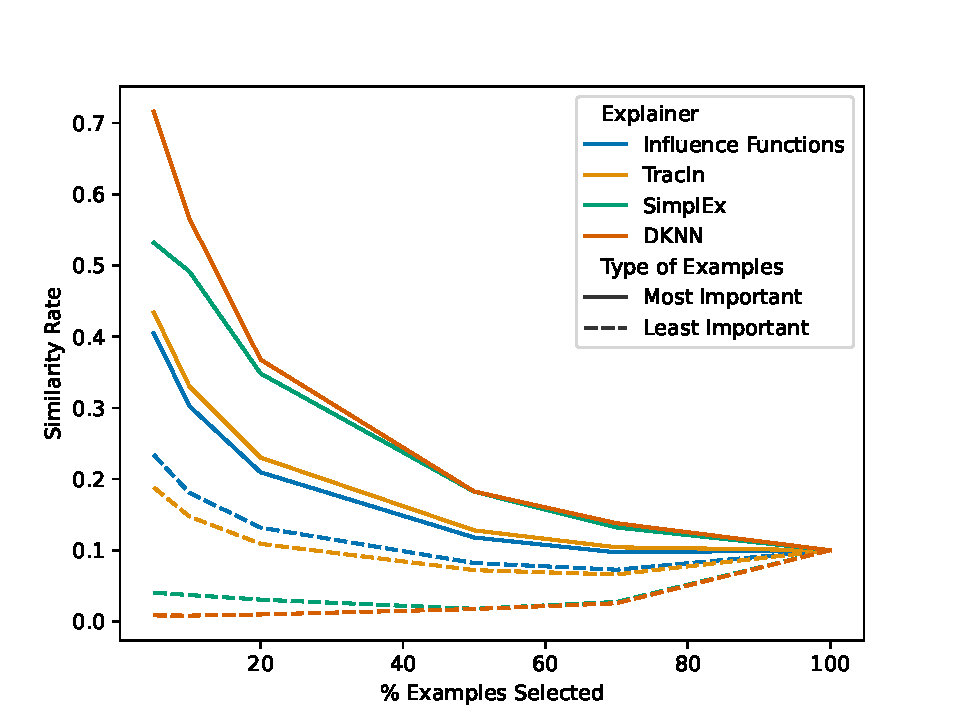
\includegraphics[width=1\linewidth]{img/og/mnist_similarity_rates}
            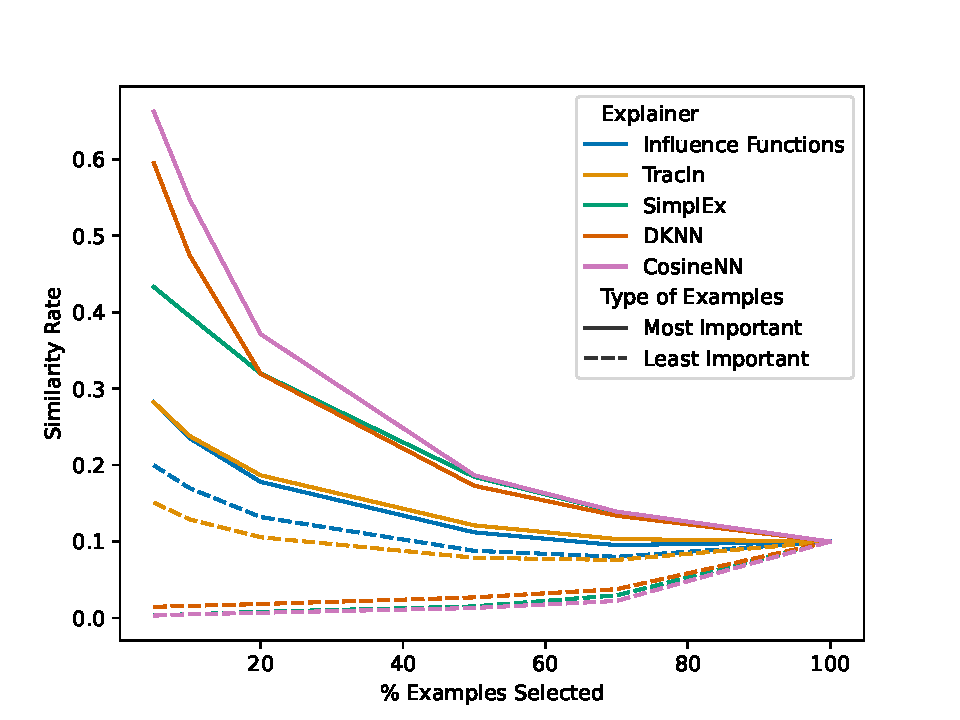
\includegraphics[width=1\linewidth]{img/extra/mnist_example_similarity_rates.pdf}
		\end{minipage}%
	}%
	\subfigure[ECG5000]{
		\begin{minipage}[t]{.25\linewidth}
			\centering
			%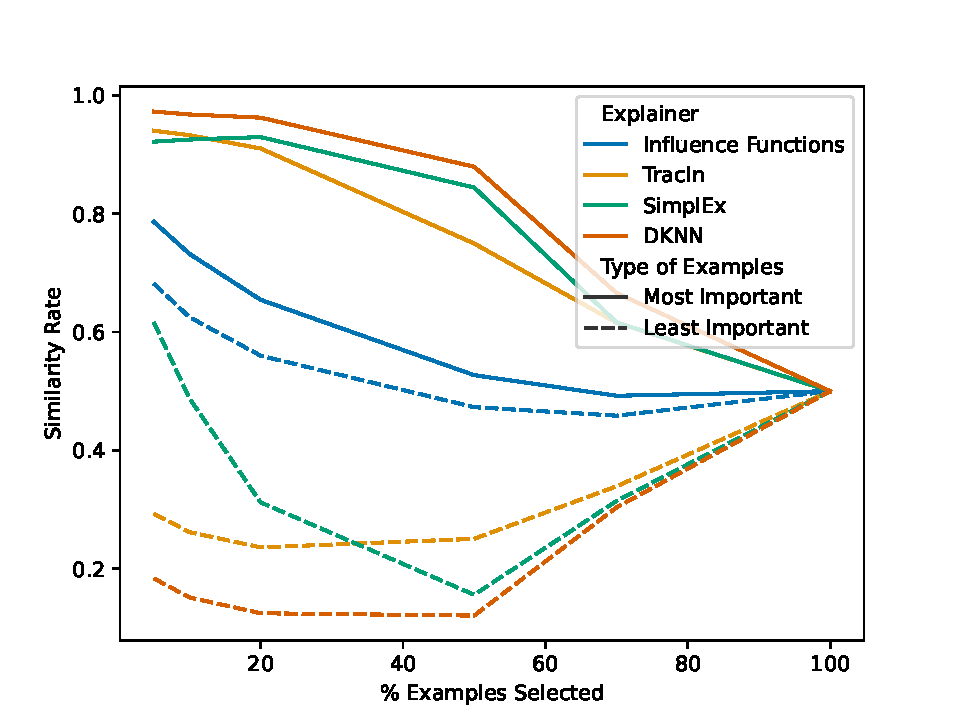
\includegraphics[width=1\linewidth]{img/og/ecg5000_similarity_rates}
            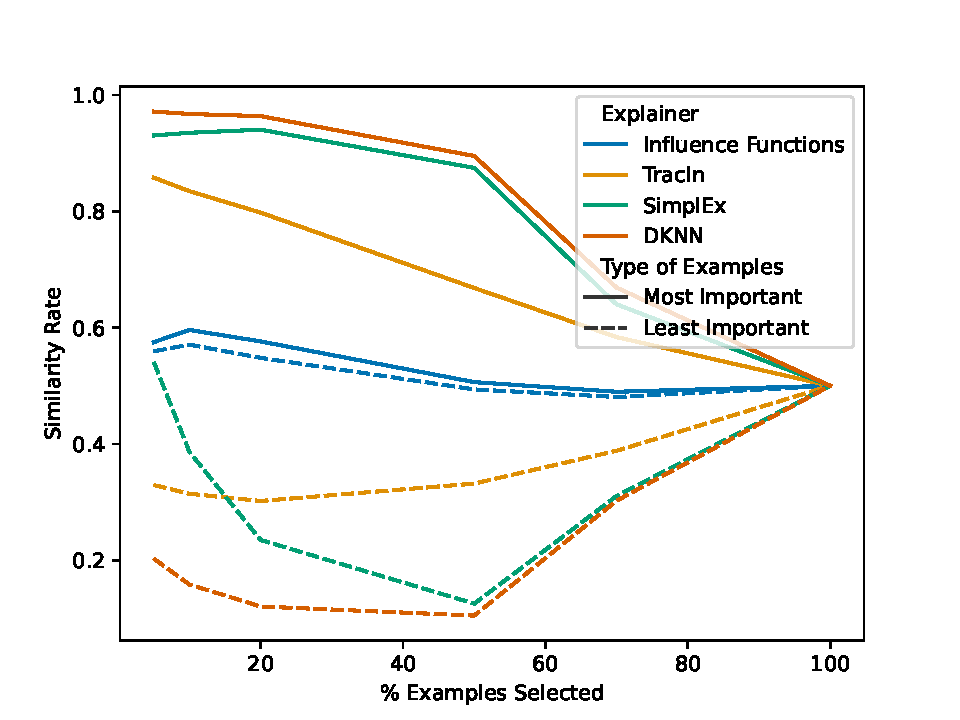
\includegraphics[width=1\linewidth]{img/rp/ecg5000_similarity_rates}
		\end{minipage}%
	}%
	\subfigure[CIFAR-10]{
		\begin{minipage}[t]{.25\linewidth}
			\centering
			%\includegraphics[width=1\linewidth]{img/og/cifar10_similarity_rates}
            \includegraphics[width=1\linewidth]{img/extra/cifar10_similarity_rates.pdf}
		\end{minipage}%
	}%
    \subfigure[CIFAR-100]{
		\begin{minipage}[t]{.25\linewidth}
			\centering
			%\includegraphics[width=1\linewidth]{img/og/cifar10_similarity_rates}
            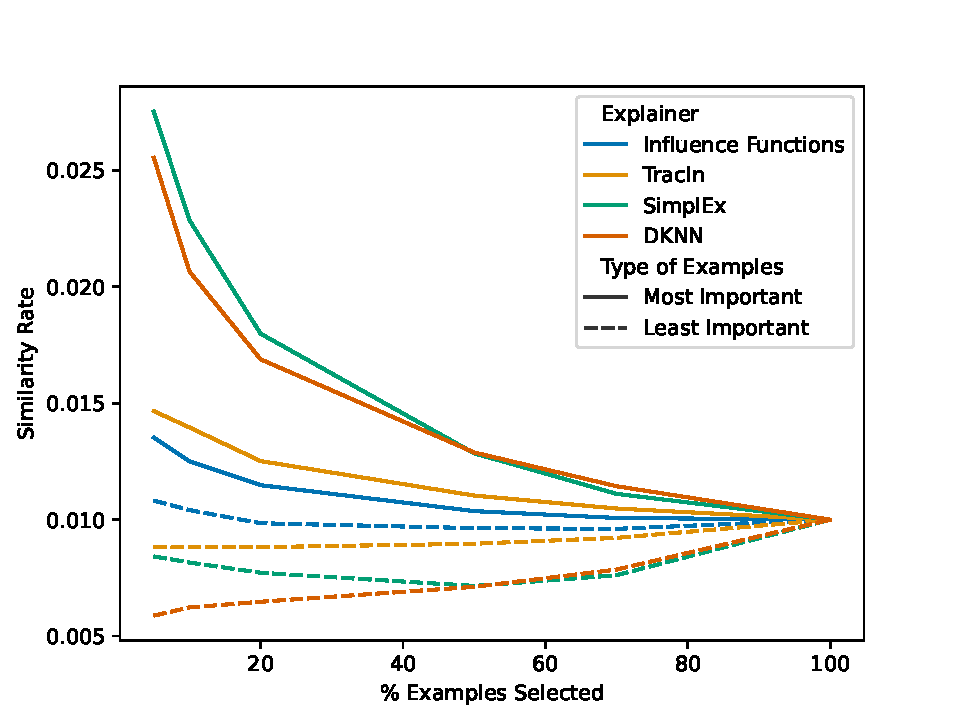
\includegraphics[width=1\linewidth]{img/extra/cifar100_similarity_rates.pdf}
		\end{minipage}%
	}%
	\vspace{-0.1in}
	\caption{Consistency check for label-free example importance. Each solid line shows how the similarity rate changes as we calculate it over some percentage of the highest-ranked training examples, for each choice of label-free example importance metric. The dotted lines show what happens if we start with the bottom-ranked samples instead.}
	\label{fig:cons_examples}
	\vspace{-0.1in}
\end{figure*}

\subsubsection{Claim 2.1 - Correlation of feature importance across tasks}

Using the MNIST dataset, we found nearly identical results to \citet{crabbe2022label} when measuring the correlations of feature importance across different tasks. All model pairs showed a modest correlation  and had a small standard error across runs (Table 1a). We found very similar results when we repeated the experiment on CIFAR-10 and CIFAR-100.

\begin{table}[]
	\begin{center}
		\begin{adjustbox}{width=\columnwidth}
			\begin{small}
				\begin{sc}
					% \begin{tabular}{l|c c c c} 
					% 	\toprule
					% 	Pearson & Recon. & Denois. & Inpaint. & Classif. \\ 
					% 	\hline
					% 	Recon. &  &  &  &  \\
					% 	Denois. & $.39 \pm .01 $ &  & &  \\
					% 	Inpaint. & $.31 \pm .02 $ & $.32 \pm .01$ &  &  \\
					% 	Classif. & $.44 \pm .02$ & $.40 \pm .00$ & $.32 \pm .02$ &  \\
					% 	\bottomrule
					% \end{tabular}
                    \subfigure[saliency maps]{\begin{tabular}{l|c c c c} 
						\toprule
						Pearson & Recon. & Denois. & Inpaint. & Classif. \\ 
						\hline
					  Recon. &  &  &  &  \\
                        Denois.      & $0.41 \pm 0.02$  & & &  \\
                        Inpaint.     & $0.34 \pm 0.03$  & $0.31 \pm 0.02$ & & \\
                        Classif. & $0.44 \pm 0.02$  & $0.39 \pm 0.01$ & $0.32 \pm 0.02$ &  \\
						\bottomrule
					\end{tabular}
                    \label{tab:pretext_features_pearson}
     }              
                    \subfigure[example importance]{
                    \begin{tabular}{l|c c c c} 
						\toprule
						Pearson & Recon. & Denois. & Inpaint. & Classif. \\ 
						\hline
                        Recon. &  &  &  &  \\
                        Denois.      & $0.1 \pm 0.02$   &  &  &   \\
                        Inpaint.     & $0.06 \pm 0.02$  & $0.1 \pm 0.04$ &  &  \\
                        Classif. & $0.06 \pm 0.02$  & $0.07 \pm 0.01$ & $0.06 \pm 0.03$ &  \\
						\bottomrule
					\end{tabular}
     \label{tab:pretext_examples_pearson}
     }
				\end{sc}
			\end{small}	
		\end{adjustbox}
	\end{center}
	\vskip -0.1in
        \caption{Pearson correlation for saliency maps and example importance (avg +/- std) between different pretext tasks on MNIST.}
        \vspace{-0.1in}
        
\end{table}

\subsubsection{Claim 2.2 - Correlation of example importance across tasks}

We also found nearly identical results to \citet{crabbe2022label} when measuring correlations of example importance across different tasks using the MNIST data (Table 1b). All model pairs showed a low correlation in example importance (0.06 to 0.1) and a low standard deviation across runs. 

\vspace{1em}

However, we found substantially different trends when we repeated the experiment on CIFAR-10 and CIFAR-100, see Table \ref{tab:extra_result_cifar_example} and \ref{tab:extra_result_cifar_saliency}. On these datasets, latent representations trained for separate unsupervised tasks had a high correlation ($\textasciitilde$ 0.9) to each other, but all had low correlation to the representations trained with the supervised task ($\textasciitilde$ 0.13).

% \begin{table}[]
	
	\vskip 0.05in
	\begin{center}
		\begin{adjustbox}{width=.5\columnwidth}
			\begin{small}
				\begin{sc}
					% \begin{tabular}{l|c c c c} 
					% 	\toprule
					% 	Pearson & Recon. & Denois. & Inpaint. & Classif. \\ 
					% 	\hline
					% 	Recon. &  &  &  &  \\
					% 	Denois.     & $.10 \pm .04$   &  &  &   \\
					% 	Inpaint.     & $.11 \pm .03$  & $.12 \pm .03$ &  &  \\
					% 	Classif. & $.07 \pm .03$  & $.06 \pm .02$ & $.07 \pm .01$ &   \\
					% 	\bottomrule
					% \end{tabular}
                    \begin{tabular}{l|c c c c} 
						\toprule
						Pearson & Recon. & Denois. & Inpaint. & Classif. \\ 
						\hline
                        Recon. &  &  &  &  \\
                        Denois.      & $0.12 \pm 0.03$  &  &  &   \\
                        Inpaint.     & $0.11 \pm 0.07$  & $0.12 \pm 0.06$ &  &  \\
                        Classif. & $0.09 \pm 0.02$  & $0.09 \pm 0.02$ & $0.08 \pm 0.04$ &  \\
						\bottomrule
					\end{tabular}
				\end{sc}
			\end{small}	
		\end{adjustbox}
	\end{center}
        \caption{Pearson correlation for example importance (avg +/- std). %The left table shows the original paper and the right table the reproduction.
        }
        \label{tab:pretext_examples_pearson}
\vspace{0in}
\end{table}

\subsubsection{Claim 3 - disentanglement of VAE}

Our results supported their claim that increasing the strength of the disentanglement regularisation parameter ($\beta$) does not decrease correlation across feature maps in either $\beta-$ or TC-VAEs. Although our results did not match theirs perfectly, we were satisfied that they exhibited the same trends, and the same rough distribution of the Pearson statistic (Figure\ref{fig:vae_pearson}). While our Lucid visualisations showed some interesting patters, they did not provide any insight into the relationship between increased $\beta$ and the Pearson correlations (Figure \ref{fig:lucid}).

\begin{figure*}[h] 
	\vspace{-0.1in}
	\centering
	\subfigure[MNIST]{
		\begin{minipage}[t]{0.35\linewidth}
			\centering
			%\includegraphics[width=\linewidth]{img/og/pearson_vae_mnist}
            \includegraphics[width=\linewidth]{img/rp/pearson_vae_mnist2}
		\end{minipage}
	}%
	\subfigure[dSprites]{
		\begin{minipage}[t]{0.35\linewidth}
			\centering
			%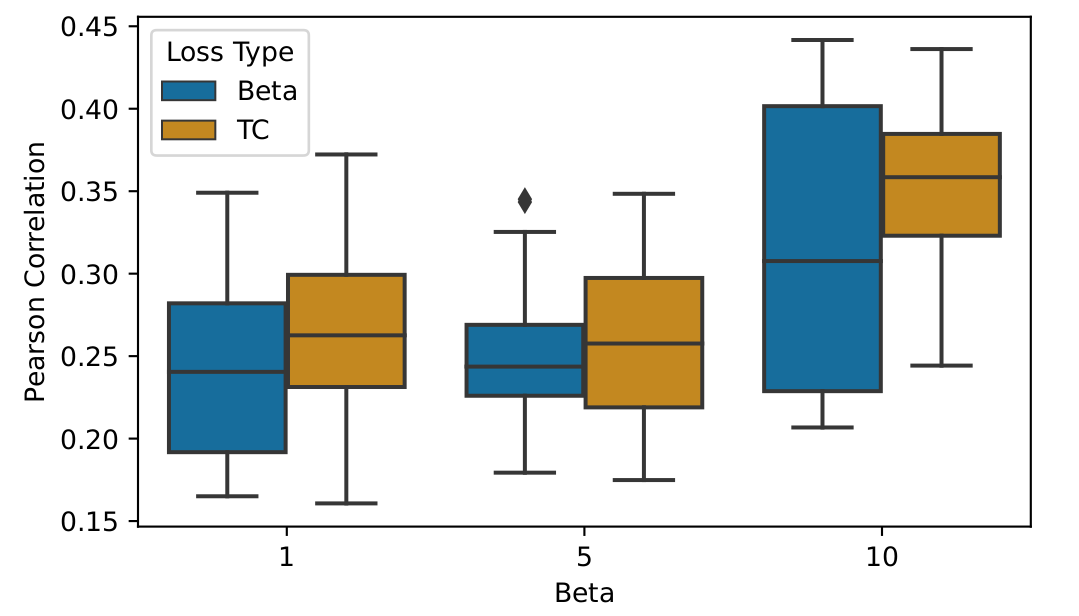
\includegraphics[width=\linewidth]{img/og/pearson_vae_dsprites}
            \includegraphics[width=\linewidth]{img/rp/pearson_vae_dsprites2}
		\end{minipage}
	}
	\vspace{-0.1in}
	\caption{Pearson correlation between feature importance scores of pairs of latent units for different values of $\beta$.}
	\label{fig:vae_pearson}
	\vspace{-0.1in}	
\end{figure*}

\subsection{Results beyond original paper}
%Often papers don't include enough information to fully specify their experiments, so some additional experimentation may be necessary. For example, it might be the case that batch size was not specified, and so different batch sizes need to be evaluated to reproduce the original results. Include the results of any additional experiments here. Note: this won't be necessary for all reproductions.
 
\begin{table}[h]
	\vskip 0.05in
	\begin{center}
		\begin{adjustbox}{width=\columnwidth}
			\begin{small}
				\begin{sc}
                    \subfigure[CIFAR-10]{
					\begin{tabular}{l|c c c c} 
						\toprule
						Pearson & Recon. & Denois. & Inpaint. & Classif. \\ 
						\hline
						Recon. & & & &  \\
                            Denois.      & $0.88 \pm 0.07$  & & &  \\
                            Inpaint.     & $0.92 \pm 0.03$  & $0.9 \pm 0.03$ & &  \\
                            Classif. & $0.16 \pm 0.02$  & $0.15 \pm 0.01$ & $0.15 \pm 0.02$ &    \\
						\bottomrule
					\end{tabular}
     }
                    \subfigure[CIFAR-100]{
                    \begin{tabular}{l|c c c c} 
						\toprule
						Pearson & Recon. & Denois. & Inpaint. & Classif. \\ 
						\hline
                        Recon. &  &  &  &  \\
                        Denois.      & $0.91 \pm 0.07$  &  &  &   \\
                        Inpaint.     & $0.89 \pm 0.03$  & $0.93 \pm 0.02$ &  &  \\
                        Classif. & $0.2 \pm 0.02$   & $0.2 \pm 0.02$  & $0.19 \pm 0.02$ &  \\
						\bottomrule
					\end{tabular}
     }
				\end{sc}
			\end{small}	
		\end{adjustbox}
	\end{center}
        \caption{Pearson correlation of example importance (avg +/- std) across different pretext tasks.}
        \label{tab:extra_result_cifar_example}
\vspace{0in}
\end{table}

\begin{table}[h]
	\vskip 0.05in
	\begin{center}
		\begin{adjustbox}{width=\columnwidth}
			\begin{small}
				\begin{sc}
                \subfigure[CIFAR-10]{
					\begin{tabular}{l|c c c c} 
						\toprule
						Pearson & Recon. & Denois. & Inpaint. & Classif. \\ 
						\hline
						Recon. & & & &  \\
                            Denois.      & $0.29 \pm 0.11$  & & &  \\
                            Inpaint.     & $0.3 \pm 0.04$   & $0.28 \pm 0.03$ & &  \\
                            Classif. & $0.19 \pm 0.01$  & $0.21 \pm 0.02$ & $0.18 \pm 0.02$ &    \\
						\bottomrule
					\end{tabular}
     }
                \subfigure[CIFAR-100]{
                    \begin{tabular}{l|c c c c} 
						\toprule
						Pearson & Recon. & Denois. & Inpaint. & Classif. \\ 
						\hline
                        Recon. &  &  &  &  \\
                        Denois.      & $0.35 \pm 0.08$  &  &  &   \\
                        Inpaint.     & $0.31 \pm 0.05$  & $0.42 \pm 0.07$ &  &  \\
                        Classif. & $0.21 \pm 0.01$  & $0.22 \pm 0.01$ & $0.2 \pm 0.01$ &  \\
						\bottomrule
					\end{tabular}
     }
				\end{sc}
			\end{small}	
		\end{adjustbox}
	\end{center}
        \caption{Pearson correlation of feature importance (mean $\pm$ standard deviation) across different pretext tasks for CIFAR10 and CIFAR100.}
        \label{tab:extra_result_cifar_saliency}
\vspace{0in}
\end{table}

% \begin{tabular}{lllll}
% \hline
%                 & Reconstruction   & Denoising       & Inpainting      & Classification   \\
% \hline
%  Reconstruction & $1.0 \pm 0.0$    & $0.26 \pm 0.05$ & $0.26 \pm 0.04$ & $0.19 \pm 0.01$  \\
%  Denoising      & $0.26 \pm 0.05$  & $1.0 \pm 0.0$   & $0.24 \pm 0.03$ & $0.19 \pm 0.03$  \\
%  Inpainting     & $0.26 \pm 0.04$  & $0.24 \pm 0.03$ & $1.0 \pm 0.0$   & $0.18 \pm 0.06$  \\
%  Classification & $0.19 \pm 0.01$  & $0.19 \pm 0.03$ & $0.18 \pm 0.06$ & $1.0 \pm 0.0$    \\
% \hline
% \end{tabular}

% % Saliency map pearsonn corr for cifar-10

% \begin{tabular}{lllll}
% \hline
%                 & Reconstruction   & Denoising       & Inpainting      & Classification   \\
% \hline
%  Reconstruction & $1.0 \pm 0.0$    & $0.3 \pm 0.03$  & $0.25 \pm 0.03$ & $0.19 \pm 0.04$  \\
%  Denoising      & $0.3 \pm 0.03$   & $1.0 \pm 0.0$   & $0.32 \pm 0.07$ & $0.23 \pm 0.02$  \\
%  Inpainting     & $0.25 \pm 0.03$  & $0.32 \pm 0.07$ & $1.0 \pm 0.0$   & $0.2 \pm 0.03$   \\
%  Classification & $0.19 \pm 0.04$  & $0.23 \pm 0.02$ & $0.2 \pm 0.03$  & $1.0 \pm 0.0$    \\
% \hline
% \end{tabular}

% Saliency maps pearsson corr for cifar-100


% The qualitative results are visualized in Appendix \ref{sec:vae_vs_classifier}.

\subsubsection{Comparison of Unsupervised and Supervised Feature Importance}

% \begin{figure}[h]
%     \centering
%     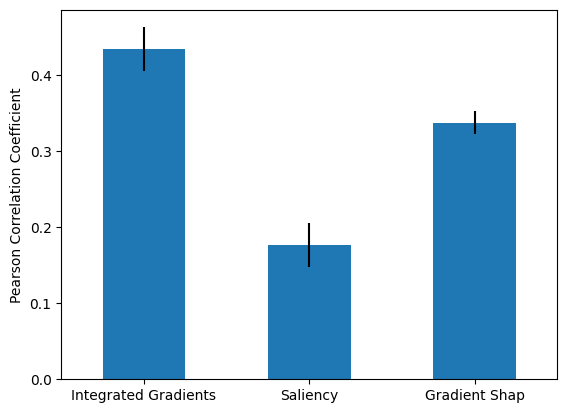
\includegraphics[scale=0.5]{figures_n_tables/add_results_pearson_enc_dec.png}
%     \caption{Pearson correlation between feature importance values of encoder and encoder/decoder architectures}
%     \label{fig:enc_dec_per}
% \end{figure}w

We found that there was at best a moderate correlation between feature importance for the latent space encoder and the full model (see figure \ref{fig:enc_dec_per}). The Pearson correlation coefficients were much higher for Integrated gradients ($\textasciitilde 0.45$) and gradient SHAP ($ \textasciitilde 0.35$) than for Saliency ($\textasciitilde0.2$). There was very little variation in the strength of correlation between different runs.

% \subsubsection{Additional Result 2 - Lucid}

% In order to understand why the correlation of features increase when increasing $\beta$ in $\beta$-VAE networks, we visualized each latent unit with Lucid \cite{olah2017feature}. The results can be seen on Figure \ref{fig:lucid}. We found that $\beta$-VAE networks with low $\beta$ coefficient focuses more on tiny details, the texture of the data. Increasing $\beta$ makes the latent units represent a larger coherent group of pixels.


% \begin{figure}[h]
%     \centering
%     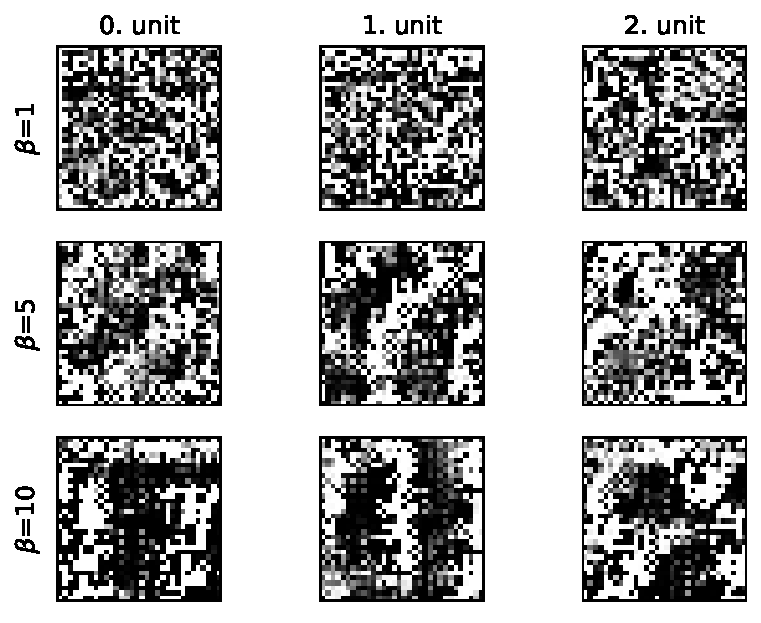
\includegraphics[scale=0.5]{img/extra/lucid.pdf}
%     \caption{Lucid visualization of the 3 latent unit across the different $\beta$-VAE networks.}
%     \label{fig:lucid}
% \end{figure}

\begin{figure*}[]
    \begin{minipage}[]{0.45\textwidth}
    \centering
        %\includegraphics[width=\linewidth]    
        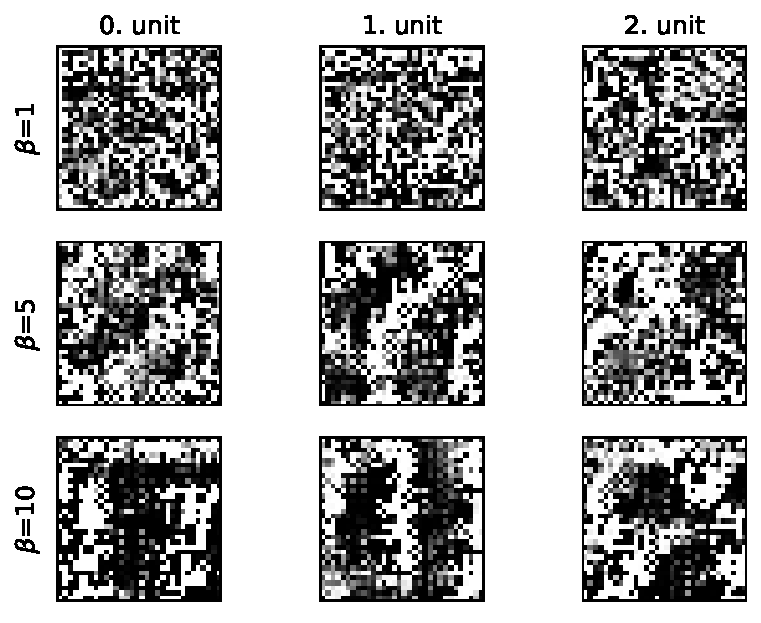
\includegraphics[width=1\textwidth]
        {img/extra/lucid.pdf}   
        \caption{Lucid visualization of the 3 latent unit across the different $\beta$-VAE networks.}
        \label{fig:lucid}
    \end{minipage}%
\hspace{2em}
    \begin{minipage}[]{0.45\textwidth}
    \centering
        %\includegraphics[width=\linewidth]
        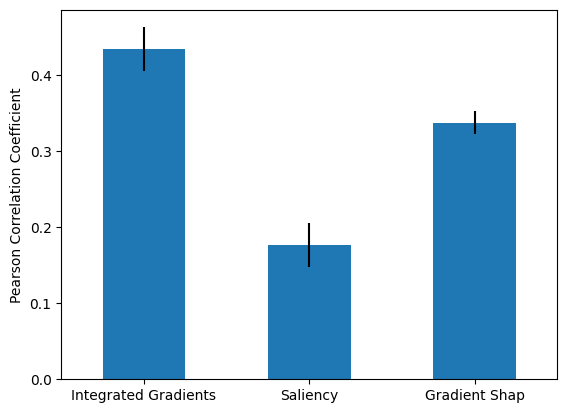
\includegraphics[width=1\textwidth]{figures_n_tables/add_results_pearson_enc_dec.png}
        \caption{Pearson correlation between feature importance values of a full classifier and its constituent latent encoder. Each value is the mean across 5 runs, shown with a 95\% confidence interval.}
        \label{fig:enc_dec_per}
    \end{minipage}%
\end{figure*}


\section{Discussion}
\label{sec:discussion}
\subsection{Reproducibility}
Overall, our reproducibility study shows that all the claims of  \textit{Label-Free Explainability for Unsupervised Models} hold. Although we could not match all their results exactly, we were satisfied that we replicated the major trends for all claims and datsasets. We found that their claims about the consistency of their methods (1.1 and 1.2) generalised well to the CIFAR-100 dataset. This indicates that the author’s proposed ‘label-free’ methods can be useful on more complex datasets than those that they originally used.

However, we found substantially different results when testing the claim (2.2) about correlations between example importance scores between latent representations using CIFAR-10 and CIFAR-100. On these more complex datasets, there was a much clearer divide between latent representations trained with and without label information. We conjecture that supervision signals have a larger impact on latent representations on more complex data, although we leave it to future work to test this more rigorously.


\subsection{Are unsupervised methods consistent with supervised ones?}
We found that there was at most a moderate correlation between the feature importance values assigned to a model and its constituent latent space encoder. While their initial experiments showed that their methods were ‘consistent’, this was only defined based on properties of the latent space, and not in terms of the application of that latent representation to a downstream task. Hence, ours is an important finding, because it shows that the ‘label-free’ feature importance values do not necessarily align with a semantically meaningful definition of importance, even when the encoder and decoder were trained together. Therefore, we recommend that in applications where an accurate representation of feature importance is essential, the label-free methods should not be substituted for label-based ones. An obvious avenue for future work is to see whether this same problem afflicts label-free example importance methods.


\subsection{What was easy}

The authors created a publicly available repository which contained code for training models, running experiments, and generating the figures and tables. We found it straightforward to use this code to replicate their experiments. Overall, the authors did an excellent job of making their work reproducible.

\vspace{1em}

Additionally, the paper was very precise in describing how their approach extended on the existing literature. We found there was no ambiguity in the mathematical details of their proposed method, and could have easily implemented it ourselves if that had been required.

\subsection{What was difficult}

Although their codebase was easy to use end-to-end, it was occasionally difficult to read and validate that the code was bug free. We believe that the readability could have been improved by consolidating the experiment code into classes that were shared between experiments for the different datasets.

\subsection{Communication with original authors}
We contacted the authors of the paper via email, to ask about the motivation behind their choice of kernel in DKNN (to which they responded they used it because it is a standard choice), and why in the computation of the saliency maps the features are multiplied with their latent values in the code (to which they responded that it was to preserve consistency with earlier methods, despite not being strictly necessary).


\section{Acknowledgment}

This work was partially supported by the Hungarian Ministry of Innovation and Technology NRDI Office within the framework of the Artificial Intelligence National Laboratory Program.